%% [migrated] heading absorbed into chapter wrapper: Scalar Fields
 
\section{Scalar fields on a lattice geometry}

\begin{itemize}
  \item We consider a real scalar field theory with mass \(m\) and Lagrangian density
\end{itemize}
\begin{equation}
\begin{aligned}
{\cal L} & =\frac{1}{2} \partial_{\mu} \varphi \partial^{\mu} \varphi-\frac{m^{2}}{2} \varphi^{2}-V(\varphi) \\
& =\frac{1}{2} \partial_{0} \varphi \partial^{0} \varphi-\frac{1}{2} \vec{\nabla} \varphi \cdot \vec{\nabla} \varphi-\frac{m^{2}}{2} \varphi^{2}-V(\varphi)
\end{aligned}
\end{equation}
where $\varphi=\varphi(\vec{x}, t) $
[cf Euclidean \(\left.{\cal L}_{E}=-\frac{1}{2} \partial_{\mu} \phi \partial_{\mu} \phi-\frac{m^{2}}{2} \varphi^{2}-V(\varphi)\right]\)

\begin{itemize}
  \item The action 
  \begin{equation}
      S=\int d^{d} \vec{x} d t \mathcal{L}(\vec{x}, t)
  \end{equation} where $d$ is the number of spatial dimensions
  \item We can quantise the theory by promoting fields to operators \(\hat{\varphi}\) and introduce canonically conjugate momenta \(\hat{\pi}=\hat{\dot\varphi}\) with \([\hat{\varphi}(\vec{x}), \hat{\pi}(\vec{y})]=i \delta^{d}(\vec{x}-\vec{y})\)  leading to a Hamiltonian

\begin{equation}
\begin{aligned}
\hat{H} & =\int d^{d} x(\hat{\pi} \hat{\dot{\varphi}}-{\cal L}) \\
& =\int d^{d} x\left(\frac{1}{2} \hat{\pi}^{2}+\frac{1}{2}(\vec{\nabla} \hat{\varphi})^{2}+\frac{m^{2}}{2} \hat{\varphi}^{2}+V(\hat{\varphi})\right).
\end{aligned}
\end{equation}

  \item Following what we did for quantum mechanics, we shall discretise time but we also will discretise space
  \item Define a $Z^d$ spatial lattice of points separated by a distance $a$ (the lattice spacing)
\begin{equation}
\begin{aligned}
& \vec{x} \rightarrow a \vec{n} \quad n_{i} \in\{0,1, \ldots, N-1\},\ i\in\{1,\ldots,d\} \\
& \Rightarrow \quad \Lambda_{d}=\left\{a \vec{n}, n_{i} \in\{0,1, \ldots, N-1\}\right\}
\end{aligned}
\end{equation}

  \item Physical extent $L=Na$ in each direction and spatial volume\(V_{d}=L^{d}\)\\
  \item Assume spatially periodic boundary conditions: identify \(n_{i}=N\) with \(n_{i}=0\)
  \item Discretisation replaces derivatives by finite differences and integrals by sums, for example

\begin{equation}
\begin{aligned}
\partial_{j} \hat{\varphi}(\vec{x}) & \longrightarrow \frac{1}{2 a}[\hat{\varphi}(\vec{n}+\hat{\jmath})-\hat{\varphi}(\vec{n}-\hat{\jmath})]+\theta\left(a^{2}\right) 
 \\
\int d^{d} \vec{x} & \rightarrow a^{d} \sum_{\vec{n}=\Lambda_{d}}
\end{aligned}
\end{equation}
where $ \hat{\jmath}$ is a unit vector in the $j$ direction
but other choices of discretisation (forward/backward/higher-order differences) are possible

  \item The discretised Hamiltonian is


\begin{equation}
\hat{H}=a^{d} \sum_{\vec n \in \Lambda_{d}}\left[\frac{1}{2} \hat{\pi}(\vec{n})^{2}+\frac{1}{8 a^{2}} \sum_{j=1}^{d}(\hat{\varphi}(\vec{n}+\hat{j})-\hat{\varphi}(\vec{n}-\hat{j}))^{2}+\frac{m^{2}}{2} \hat{\varphi}(\vec{n})^{2}+V(\varphi(\vec{n}))\right]
\end{equation}


  \item We can introduce eigenstates of field operators and canonical momenta\\
\begin{itemize}
     \item\(\hat{\varphi}(\vec{n})|\varphi\rangle=\varphi(\vec{n})|\varphi\rangle \quad[| \varphi\rangle\) contains information about \(\varphi\) everywhere]\\
with \begin{equation}\left\langle\varphi \mid \varphi^{\prime}\right\rangle=\delta\left(\varphi-\varphi^{\prime}\right)=\prod_{\vec{n} \in \Lambda_{d}} \delta\left(\varphi(\vec{n})-\varphi^{\prime}(\vec{n})\right)\end{equation}\\
and
\begin{equation}
\begin{aligned}
& 1=\int \mathcal{D}_{d} \varphi|\varphi\rangle\langle\varphi| \\
& \quad=\prod_{\vec{n} \in \Lambda_{d}} \int_{-\infty}^{\infty} d \varphi(\vec{n})|\varphi\rangle\langle\varphi|
\end{aligned}
\end{equation}


  \item \(\hat{\pi}(\vec{n})|\pi\rangle=\pi(\vec{n})|\pi\rangle,\left\langle\pi \mid \pi^{\prime}\right\rangle=\delta\left(\pi-\pi^{\prime}\right), 1=\int \mathcal{D}_{d} \pi|\pi\rangle\langle\pi|\)
  
\end{itemize} 
  \item Plane waves in field configuration space are given by

\begin{equation}
\langle\varphi | \pi\rangle=\left(\frac{a^{d}}{2 \pi}\right)^{N^d / 2} \exp \left[i a^{d} \sum_{\vec{n} \in \Lambda_{d}} \pi(\vec{n}) \varphi(\vec{n})\right].
\end{equation}

  \item Now let us consider imaginary time evolution as before

\begin{equation}
\exp (-\tau \hat{H})=\lim _{N_{\tau} \rightarrow \infty}(\hat{T}(\varepsilon))^{N_{T}} \quad \varepsilon=\frac{\tau}{N_{T}}
\end{equation}

with the transfer matrix operator

\begin{equation}
\hat{T}(\varepsilon)=\exp \left(-\frac{\varepsilon}{2} \hat{U}\right) \exp \left(-\varepsilon \hat{H}_{0}\right) \exp \left(-\frac{\varepsilon}{2} \hat{U}\right)
\end{equation}

for

\begin{equation}
\begin{aligned}
& \hat{H}_{0}=\frac{a^{d}}{2} \sum_{\vec{n} \in \Lambda_{d}} \hat{\pi}(\vec{n})^{2} \\
& \hat{U}=a^{d} \sum_{\vec{n} \in \Lambda_{d}}\left\{\frac{1}{8a^{2}} \sum_{j=1}^{d}\left(\hat{\varphi}(\vec{n}+\hat{j})-\hat{\varphi}(\vec{n}-\hat{j})\right)^{2}+\frac{m^{2}}{2} \hat{\varphi}(\vec{n})^{2}+V(\hat\varphi(\vec{n}))\right\}
\end{aligned}
\end{equation}


  \item We label field eigenvalues at a given time as \(\left|\varphi_{s}\right\rangle\) for \(\tau=s \varepsilon\) with eigenvalues

\begin{equation}
\hat{\varphi}(\vec{n})\left|\varphi_{s}\right\rangle=\varphi_{s}(\vec{n})\left|\varphi_{s}\right\rangle
\end{equation}

that are the field on the given timeslice.

  \item We can evaluate an infinitesimal time evolution

\begin{equation}
\begin{aligned}
& \left\langle\varphi_{s+1}\right| \hat T(\varepsilon)\left|\varphi_{s}\right\rangle=\left\langle\varphi_{s+1}\right| e^{-\frac{\varepsilon}{2} \hat{U}} e^{-\varepsilon \hat{H}_{0}} e^{-\frac{\varepsilon}{2} \hat{U}}\left|\varphi_{s}\right\rangle \\
& \quad=\exp \left\{-\frac{\varepsilon}{2}\left[U\left(\varphi_{s+1}\right)+U\left(\varphi_{s}\right)\right]\right\}\langle\varphi_{s+1} \mid e^{-\varepsilon \hat{H}_{0}} \int \mathcal{D}_{d} \pi | \pi\rangle\left\langle\pi \mid \varphi_{s}\right\rangle
\end{aligned}
\end{equation}
where $U(\varphi)$ is given by action of $\hat U$ on field eigenstate $\left|\varphi\right\rangle$.
The remaining matrix element is
\begin{equation}
\begin{aligned}
\langle\varphi_{s+1} \mid e^{-\varepsilon \hat{H}_{0}} \int \mathcal{D}_{d} \pi | \pi\rangle\left\langle\pi \mid \varphi_{s}\right\rangle & =\int \mathcal{D}_{d} \pi\left\langle\varphi_{s+1} \mid \pi\right\rangle\left\langle\pi \mid \varphi_{s}\right\rangle \exp \left(-\frac{\varepsilon a^{d}}{2} \sum_{\vec{n} \in \Lambda_{d}} \pi(\vec{n})^{2}\right) \\
& =\int \mathcal{D}_{d} \pi \exp \left[a^{d} \sum_{\vec{n} \in \Lambda_{d}}\left\{-\frac{\varepsilon}{2} \pi^{2}(\vec{n})+i \pi(\vec{n})\left(\varphi_{s+1}(\vec{n})-\varphi_{s}(\vec{n})\right)\right\}\right] \\
& =\prod_{\vec{n} \in \Lambda_{d}}\left[\frac{a^{d}}{2 \pi} \int_{-\infty}^{\infty} d \pi(\vec{n}) \exp \left\{-\frac{\varepsilon a^{d}}{2} \pi(\vec{n})^{2}+i \pi(\vec{n})\left(\varphi_{s+1}(\vec{n})-\varphi_{s}(\vec{n})\right)\right\}\right] \\
& =\prod_{\vec{n} \in \Lambda_{d}}\left[\sqrt{\frac{a^{d}}{2 \pi \varepsilon}} \exp \left[-\frac{a^{d}}{2 \varepsilon}\left(\varphi_{s+1}(\vec{n})-\varphi_{s}(\vec{n})\right)^{2}\right]\right]
\end{aligned}
\end{equation}

and thus

\begin{equation}
\left\langle\varphi_{s+1}\right| \hat T(\varepsilon)\left|\varphi_{s}\right\rangle=C \exp\left\{-\frac{\varepsilon}{2}\left(U\left(\varphi_{s+1}\right)+U\left(\varphi_{s}\right)\right)-\frac{a^{d}}{2 \varepsilon} \sum_{\vec{n} \in \Lambda_{d}}\left(\varphi_{s+1}(\vec{n})-\varphi_{s}(\vec{n})\right)^{2}\right\}
\end{equation}

with \(C=\left(a^{d} / 2 \pi \varepsilon\right)^{N^{d} / 2}\)\\
which depends on the fields on timeslice \(s\) and \(s+1\)

  \item We can use this to construct the partition function or correlation functions (with $\tau=\varepsilon N_{\tau}$, $t=\varepsilon N_{t}$)

\begin{equation}
\begin{aligned}
X =&\operatorname{Tr}\left[e^{-\tau \hat H} \hat{\theta}_{2}(t) \hat{\theta}_{1}(0)\right]=\operatorname{Tr}\left[e^{-(\tau-t) \hat{H}} \hat{\theta}_{2}(0) e^{-t \hat{H}} \hat{\theta}_{1}(0)\right] \\
=&\lim _{\substack{N_{\tau} \rightarrow \infty \\
N_{t} \rightarrow \infty}} \operatorname{Tr}\left[\hat{T}(\varepsilon)^{N_{\tau}-N_{t}} \hat{\theta}_{2} \hat{T}(\varepsilon)^{N_{t}} \hat{\theta}_{1}\right]  \\
=&\lim _{\substack{N_{\tau} \rightarrow \infty \\
N_{t} \rightarrow \infty}} \int \mathcal{D} \varphi_{0} \ldots \mathcal{D} \varphi_{N_{\tau}-1} \mathcal{D} \widetilde{\varphi}_{1} \mathcal{D} \widetilde{\varphi}_{2}\left\langle\varphi_{0}\right| \hat{T}(\varepsilon)\left|\varphi_{N_{\tau}-1}\right\rangle\left\langle\varphi_{N_{\tau}-1}\right| \hat{T}(\varepsilon)\left|\varphi_{N_{\tau}-2}\right\rangle \ldots \\
&\qquad  \ldots\left\langle\varphi_{N_{t+1}}\right| \hat{T}(\varepsilon)\left|\widetilde{\varphi}_{2}\right\rangle\left\langle\widetilde{\varphi}_{2}\right| \hat{\theta}_{2}\left|\varphi_{N_{t}}\right\rangle\left\langle\varphi_{N_{t}}\right| \hat{T}(\varepsilon)\left|\varphi_{N_{t}-1}\right\rangle \ldots . \\
& \qquad \ldots\left\langle\varphi_{1}\right| \hat{\tau}(\varepsilon)\left|\widetilde{\varphi}_{1}\right\rangle\left\langle\widetilde{\varphi}_{1}\right| \hat{\theta}_{1}\left|\varphi_{0}\right\rangle
\end{aligned}
\end{equation}


Since \(\hat{\theta}_{i}\) will be a function of the field operators (e.g. $\hat{\theta_i} = \hat{\varphi}^3$) then

\begin{equation}
\left\langle\tilde{\varphi}_{j}\right| \hat{\theta}\left|\varphi_{k}\right\rangle=\theta\left(\varphi_{k}\right)\left\langle\tilde{\varphi}_{j} \mid \varphi_{k}\right\rangle=\theta\left(\varphi_{k}\right) \delta\left(\tilde{\varphi}_{j}-\varphi_{k}\right)
\end{equation}

Thus

\begin{equation}
\begin{aligned}
 X=&\lim _{O\ll N_{t}\ll N_{\tau}} C^{N_\tau} \int \mathcal{D} \varphi_{0} \ldots \mathcal{D} \varphi_{N_{\tau-1}} \theta_{2}\left(\varphi_{N_{t}}\right) \theta_{1}\left(\varphi_{0}\right) \times \\
& \qquad \qquad\times \exp \left[-\frac{\varepsilon}{2}\left\{U\left(\varphi_{0}\right)+U\left(\varphi_{N_{\tau} - 1}\right)\right\}-\frac{a^{d}}{2 \varepsilon} \sum_{\vec{n}\in\Lambda_d} \left(\varphi_{0}(\vec{n})-\varphi_{N_{\tau}-1}(\vec{n})\right)^{2}\right] \\
& \qquad \qquad \times \cdots \times \exp \left[-\frac{\varepsilon}{2}\left\{U\left(\varphi_{1}\right)+U\left(\varphi_{0}\right)\right\}-\frac{a^{d}}{2 \varepsilon} \sum_{\vec{n} \in \Lambda_{d}}\left(\varphi_{1}(\vec{n})-\varphi_{0}(\vec{n})\right)^{2}\right] \\
=&\lim _{0\ll N_{t} \ll N_{\tau}} C^{N_{\tau}} \int \mathcal{D} \varphi_{0} \ldots \mathcal{D} \varphi_{N_{\tau}-1} \theta_{2}\left(\varphi_{N_{t}}\right) \theta_{1}\left(\varphi_{0}\right) \exp \left(-S_{E}[\varphi]\right)
\end{aligned}
\end{equation}

with

\begin{equation}
S_{\varepsilon}[\varphi]=\frac{a^{d}}{2 \varepsilon} \sum_{s=0}^{N_{\tau}-1} \sum_{\vec{n} \in \Lambda_d}\left[\varphi_{s+1}(\vec{n})-\varphi_{s}(\vec{n})\right]^{2}+\varepsilon \sum_{s=0}^{N_{\tau}-1} U\left(\varphi_{s}\right)
\end{equation}

where we assume \(\varphi_{N_{\tau}}=\varphi_{0}\) (periodic in time)

  \item If we define a \(d+1\) dimensional lattice with an isotropic spacing

\begin{equation}
\Lambda=\left\{a\left(\vec{n}, n_{4}\right) \mid n_{i} \in\{0,1, \ldots, N-1\} \forall i=1, \ldots, d ; n_{4} \in\left\{0,1, \ldots N_{\tau}-1\right\}\right\}
\end{equation}

then we can write

\begin{equation}
\begin{aligned}
 S_{E}[\varphi]=&a^{d+1} \sum_{\left(\vec{n}, n_{4}\right) \in \Lambda}\left\{\frac{1}{2a^2}\left[\varphi_{n_{4}+1}(\vec{n})-\varphi_{n_{4}}(\vec{n})\right]^{2}+\frac{1}{8 a^{2}} \sum_{j=1}^{d}\left[\varphi_{n_{4}}(\vec{n}+\hat{j})-\varphi_{n_{4}}(\vec{n}-\hat{\jmath})\right]^{2}\right. \\
&\hspace*{2cm}\left.+\frac{m^{2}}{2} \varphi_{n_{4}}(\vec{n})^{2}+V\left(\varphi_{n_{4}}(\vec{n})\right)\right\}
\end{aligned}
\end{equation}

  \item With a small change from the central difference in space that arose from canonical quantization to a forward difference, we can make space and time symmetric

\begin{equation}
S_{\varepsilon}[\varphi]=a^{d+1} \sum_{n_{\mu} \in \Lambda}\left\{\frac{1}{2 a^{2}} \sum_{v=1}^{d_{1}+1}\left[\varphi\left(n_{\mu}+\hat{v}\right)-\varphi\left(n_{\mu}\right)\right]^{2}+\frac{m^{2}}{2} \varphi\left(n_{\mu}\right)^{2}+V\left(\varphi\left(n_{\mu}\right)\right)\right\}
\label{eq:scalar_euclidean_action}
\end{equation}

where \(\varphi\left(n_{\mu}\right)=\varphi_{n_{4}}(\vec{n})\). Note that we could also make all finite differences central differences, but that breaks reflection positivity.

  \item Defining \(\mathcal{D} \varphi=\prod_{s=0}^{N_{\tau}-1} \mathcal{D} \varphi_{s}=\prod_{s=0}^{N_{\tau}-1} \prod_{\vec{n}\in\Lambda_d} d \varphi_{s}(\vec{n})\)

\begin{equation}
\Rightarrow Z(\tau)=\operatorname{tr}\left[e^{-\tau \hat{H}}\right]=\int \mathcal{D} \varphi e^{-S_{E}[\varphi]}
\end{equation}

and e.g.

\begin{equation}
\begin{aligned}
    \langle\Omega| \hat{\theta}_{2}(t) \hat{\theta}_{1}(0)|\Omega\rangle &=\frac{1}{Z(\tau)} \operatorname{Tr}\left[e^{-\tau \hat{H}} \hat{\theta}_{2}(t) \hat{\theta}_{1}(0)\right] \\
&=\frac{1}{Z({\tau})} \int \mathcal{D} \varphi \theta_{2}(\varphi) \theta_{1}(\varphi) \exp \left[-S_{E}[\varphi]\right]
\end{aligned}
\end{equation}

\end{itemize}

\section{Relation to statistical mechanics}

\begin{itemize}
  \item The quantity \(Z(\tau)\) above was constructed with the boundary condition that \(\varphi_{N_{t}}=\varphi_{0}\) (i.e. periodic in time)\\
This was a mathematical convenience but has a close analogy with quantum statistical mechanics at non-zero temperature.
  \item If \(\beta=(k T)^{-1}\) (with \(k=\) Boltzmann's constant) then the partition function

\begin{equation}
Z(\beta)=\operatorname{tr}\left(e^{-\beta \hat H}\right)
\end{equation}

and thermal expectation values are

\begin{equation}
\langle\theta\rangle_{\beta}=\frac{1}{Z(\beta)} \operatorname{Tr}\left(e^{-\beta \hat{H}} \hat{\theta}\right)
\end{equation}

for the physical temperature \(T\) with \(\varphi(x+\beta \hat{t})=\varphi(x)\)

  \item For a lattice geometry with temporal extent \(N_{t}, \beta=a_{t} N_{t} \Rightarrow T=\frac{1}{k a_{t} N_{t}}\), where $a_t$ is the temporal lattice spacing
  \item The temperature can be varied by changing the \# of sites in the temporal direction at fixed lattice spacing \(a_{t}\)
  \item Alternatively one con consider an anisotropic discretisation which allows the spatial lattice spacing to be held fixed while the temporal extent is charges continuously for a fixed number of sites
  \item For zero-temperature physics, in which $N_t\to\infty$, any boundary conditions can be chosen and lead to effects that are suppressed as $e^{-N_t}$. For example, Dirichelet boundary conditions are sometimes used in gauge theories as they allow gauge field topology to change 
  
  \end{itemize}

\section{Free lattice scalar propagator}

\begin{itemize}
  \item Consider the action above \(\quad S_{E}[\varphi]=a^{d+1} \sum_{n_{\mu}\in\Lambda}\left\{\frac{1}{2 a^{2}} \sum_{v=1}^{d+1}\left[\varphi\left(n_{\mu}+\hat{\nu}\right)-\varphi\left(n_{\mu}\right)\right]^{2}+\frac{m^{2}}{2} \varphi\left(n_{\mu}\right)^{2}+V\left(\varphi\left(n_{\mu}\right)\right)\right\}\) with \(V=0\) in periodic boundary conditions
  \item Can rewrite in terms of a Klein-Gordon operator

\begin{equation}
\begin{aligned}
S_{E}[\varphi] & =\frac{a^{d+1}}{2} \sum_{k, l \in \Lambda} \varphi(k) D_{KG}(k, l) \varphi(l) \\
& =\frac{a^{d+1}}{2} \sum_{k, l \in \Lambda} \varphi_{k} D_{k l} \varphi_{l}
\end{aligned}
\end{equation}

with

\begin{equation}
D_{k l}=\sum_{n}\left\{\sum_{\mu}\left(\bar{\delta}_{n+ \hat{\mu}, k}-\bar{\delta}_{n, k}\right)\left(\bar{\delta}_{n+ \hat{\mu}, l}-\bar{\delta}_{n, l}\right)+m^{2} \bar{\delta}_{n, k} \bar{\delta}_{n, l}\right\}
\end{equation}

where

\begin{equation}
\bar{\delta}_{a, b}= \begin{cases}0 & a \neq b \bmod N \\ 1 & a=b \operatorname{rod} N\end{cases}
\end{equation}

  \item Let \(G\) be the inverse of \(D\)

\begin{equation}
D_{k n} G_{n l}=\bar{\delta}_{k, l}
\end{equation}

we can find \(G\) via Fourier transforms (setting \(a=1\) and using e.g. $ \delta_{n+\hat\mu, k} \delta_{n, l} e^{-i p k+i q l}=e^{i p \hat{\mu}} e^{-i p n+i q n}$)

\begin{equation}
\begin{aligned}
 D_{p,-q}&=\sum_{k, l} e^{-i p k+i q l} D_{k l}  \\
& =\sum_{n}\left[\sum_{\mu}\left(e^{-i p \hat{\mu}}-1\right)\left(e^{i q \hat{\mu}}-1\right)+m^{2}\right] e^{-i p n+i q n} \\
& =\left[\sum_{\mu}\left(e^{-i p \hat{\mu}}-1\right)\left(e^{i p \hat{\mu}}-1\right)+m^{2}\right] \bar{\delta}_{p, q} \\
& =\left[2 \sum_{\mu}\left(1-\cos p_{\mu}\right)+m^{2}\right] \bar{\delta}_{p, q}
\end{aligned}
\end{equation}

which is diagonal

\begin{equation}
\Rightarrow \quad G_{p,-q}=G_{p} \bar{\delta}_{p,q}=\frac{\bar{\delta}_{p, q}}{m^{2}+2 \sum_{\mu}\left(1-\cos p_{\mu}\right)}=\frac{\bar{\delta}_{p, q}}{m^{2}+4 \sum_{\mu} \sin ^{2} \frac{p_{\mu}}{2}}
\end{equation}

and restoring dimensional quantities

\begin{equation}
G_{p} \rightarrow a^{2} G(p) \quad G(p)=\frac{1}{m^{2}+a^{-2} \sum_{r}\left(2-2 \cos \left(a p_{\mu}\right)\right)} \xrightarrow{a \rightarrow 0} \frac{1}{\underbrace{m^{2}+p^{2}}_{\substack{\text { Euclidean free } \\ \text { propagator }}}}+\theta\left(a^{2}\right)
\end{equation}

  \item Defining the partition function with external source \(J\)

\begin{equation}
Z[J]=\int \mathcal{D} \varphi \exp \left(-S+\sum_{k} \varphi_{k} J_{k}\right)
\end{equation}

a change of variables \(\varphi_{k} \rightarrow \varphi_{k}+\sum_{n} G_{k n} J_{n}\) and completing the square leads to

\begin{equation}
\begin{aligned}
Z[J] & =\int \mathcal{D} \varphi e^{-S} \exp \left(-\frac{1}{2} J_{k} G_{k l} J_{l}\right) \\
\Rightarrow \quad\left\langle\varphi_{k} \varphi_{l}\right\rangle & =\left.\left[\frac{\partial \ln Z}{\partial J_{k} \partial J_{l}}\right]\right|_{J=0}=G_{k l}=\text { propagator }
\end{aligned}
\end{equation}

Note that under the change of variables:

\begin{equation}
\begin{aligned}
& S=\frac{1}{2} \varphi^{\prime} D \varphi^{\prime} =\frac{1}{2} \varphi D \varphi +\frac{1}{2} \varphi J+\frac{1}{2} J \varphi+J G J / 2 \\
 \Rightarrow&-S+\varphi J  =-\frac{1}{2} \varphi D \varphi-\frac{1}{2} J G J
\end{aligned}
\end{equation}

  \item Going back to position space

\begin{equation}
\begin{array}{rlrl}
G_{k l} & =\sum_{p} e^{i p(k-l)} G_{p} & k-l=(\vec{x}, t) \\
G(\vec{x}, t) & =\sum_{\vec{p}} e^{i \vec{p} \vec{x}} 
\underbrace{\int_{-\pi}^{\pi} \frac{d p_{4}}{2 \pi} \frac{e^{i p_{4} t}}{2 b-2 \cos p_{4}}}_I. & \text { assuming } N_{t} \rightarrow \infty
\end{array}
\end{equation}

with \(b=1+\frac{1}{2}\left(m^{2}+\sum_{j=1}^{d} 4 \sin ^{2} \frac{p_{j}}{2}\right)\)

Note that we have used the identity
$1-\cos \theta=2 \sin ^{2} \frac{\theta}{2}$.
To do the $p_4$ integral, write \(z=e^{i p_4}\)

\begin{equation}
\begin{aligned}
I & =\int \frac{d z}{2 \pi i} \frac{z^{t}}{2 b z-z^{2}-1} \\
& =-\oint \frac{d z}{2 \pi i} \frac{z^{t}}{(z-z+)(z-z-)}
\end{aligned}
\end{equation}

where \(z_{ \pm}=b \pm \sqrt{b^{2}-1} \in \mathbb{R}\), \(z_- = e^{-\omega}, b = \cosh \omega\) so \(e^{-\omega} = b - \sqrt{b^2 - 1}\), and the contour encloses $z_-$ but not $z_+$, as shown in the figure.

We now use
\begin{equation}
\frac{d z}{d p_{4}}=i z \quad d p_{4}=\frac{d z}{i z} \quad \cos p_4 = \frac{1}{z}\left(z + \frac{1}{z}\right)
\end{equation}

\begin{center}

\includegraphics[width=0.3\textwidth]{fig-notes-001.jpg}
\end{center}
to evaluate using the residue theorem, this gives\footnote{The following identities are used to simplify
\begin{equation}
    \begin{aligned}
z_- - z_+ &= -2 \sqrt{b^2-1}=-2 \sinh \omega\\
\cosh^2 x - 1 &= \sinh^2 x\\
e^{-x} &= \cosh x - \sinh x
\end{aligned}
\end{equation}}
%
\begin{align}
I&=\frac{e^{-\omega t}}{2 \sinh \omega} \\
\Rightarrow G(\vec{x}, t) &= \sum_{\vec{p}}\frac{e^{i \vec{p} \vec{x} - \omega t}}{2 \sinh \omega}
\end{align}


where \(\omega=\omega(\vec{p}) \xrightarrow[a \rightarrow 0]{ } \sqrt{m^{2}+\vec{p}^{2}}\) and consequently

\begin{equation}
G(\vec{x}, t \rightarrow \infty) \sim e^{-m t}
\end{equation}

\item The behavior of $\omega(\vec{p})$ for zero and nonzero masses in the continuum, and for nonzero masses at $a\ne 0$, is shown in the figure.


\includegraphics[width=0.4\textwidth, center]{fig-notes-002.jpg}\\

\end{itemize}




\section{The transfer matrix \& reflection positivity}
The transfer matrix introduced above defines the time evolution of time-sliced fields

\begin{itemize}
  \item In the \(d+1\) dimensional setting, time-sliced fields are
\end{itemize}

\begin{equation}
\phi_{s}=\left\{\varphi(x) \mid x_{4}=s\right\}
\end{equation}

and the Euclidean action (Eq.~\eqref{eq:scalar_euclidean_action}) can be separated as

\begin{equation}
S_{E}(\varphi)=\sum_{s=0}^{N_t-1} L\left[\phi_{s+1}, \phi_{s}\right]
\label{eq:S_E2}
\end{equation}

with

\begin{equation}
L\left[\phi_{s+1}, \phi_{s}\right]=\sum_{\vec{n}\in \Lambda_d} \frac{1}{2}[\varphi(\vec{n}, s+1)-\varphi(\vec{n}, s)]^{2}+\frac{1}{2}\left[\tilde{L}\left(\phi_{s+1}\right)+\tilde{L}\left(\phi_{s}\right)\right],
\end{equation}
where
\begin{equation}
 \tilde{L}\left(\phi_{s}\right)=\sum_{\vec{n} \in \Lambda_d}\left\{\frac{1}{2} \sum_{j=1}^{d}[\varphi(\vec{n}+\hat{j}, s)-\varphi(\vec{n}-\hat{j}, s)]^{2}+\frac{m^{2}}{2} \varphi(\vec{n}, s)+V(\varphi(\vec{n}, s))\right\}
\end{equation}

Note that each \(L\left[\phi_{s+1}, \phi_{s}\right]\) only depends on the neighbouring timeslice fields

The transfer matrix

\begin{equation}
T\left[\phi_{s+1}, \phi_{s}\right]=e^{-L\left[\phi_{s+1}, \phi_{s}\right]}
\end{equation}

takes states defined on one timeslice to the next.

\begin{itemize}
  \item In particular, for a wavefunction \(\Psi\left[\phi_{s}\right]\)
\end{itemize}

\begin{equation}
\Psi\left[\phi_{s+1}\right]=\int D \phi_{s} T\left[\phi_{s+1}, \phi_{s}\right] \Psi\left[\phi_{s}\right]
\end{equation}

\begin{itemize}
  \item The transfer matrix defines the lattice Hamiltonian through its matrix element or formally at an operator level
\end{itemize}

\begin{equation}
\hat{T}=\exp [-a \hat{H}]
\end{equation}

\begin{itemize}
  \item In order for a Euclidean QFT to have an analytic continuation to a well-defined Minkowski-space QFT, its Green functions (referred to as Schwinger functions) must satisfy various requirements (Osterwalder-Schrader axioms). 
  \begin{enumerate}
      \item Temperedness of Schwinger functions
      \item Euclidean covariance ($\langle {\cal O}(R\cdot x+a)\rangle=\langle {\cal O}(x)\rangle$ for $R\in SO(D),\ a\in \mathbb{R}^D$)
      \item (Reflection) positivity
      \item Symmetry: invariance under permutations
      \item Cluster property ($\underset{\lambda\to\infty}{\lim}\langle {\cal O}(\lambda a)\tilde{\cal O}(0)\rangle-\langle{\cal O}(\lambda a)\rangle\langle\tilde{\cal O}(0)\rangle\to0$)
  \end{enumerate}
  Most of these are analogous to the Wightman axioms of Minkowski field theory
  An important one related to time reversal (although Euclidean time is not special) is called reflection positivity of all Schwinger functions
[NB: for scalar theories, OS reconstruction thm details how the Minkowski space theory can be built]
  \item Euclidean time reflection is
\end{itemize}

\begin{equation}
x=\left(\vec{x}, x_{n}\right) \rightarrow \theta{x}=\theta\left(\vec{x}, x_{4}\right)=\left(\vec{x}_{1},-x_{4}\right)
\end{equation}

and for scalar fields

\begin{equation}
\begin{aligned}
& \varphi(x) \rightarrow \theta \varphi(x)=\varphi^{*}(\theta x)=\varphi^{*}\left(\vec{x},-x_{4}\right)
\end{aligned}
\end{equation}

and more generally extended by antilinearity

\begin{equation}
\begin{aligned}
& \theta(\lambda F)=\lambda^{*} \theta(F) \\
& \theta(F G)=\theta(F) \theta(G)
\end{aligned}
\end{equation}

where \(\lambda \in \mathbb{C}\) and \(F, G\) are arbitrary products of the field \(\varphi\).
%
Note that very similar results apply for gauge and fermion fields.

\begin{itemize}
  \item For
\end{itemize}

\begin{equation}
F=\sum_{j} \int d x_{1} \ldots d x_{j} f_{j}\left(x_{1}, \ldots, x_{j}\right) \varphi\left(x_{1}\right) \ldots \varphi\left(x_{j}\right)
\end{equation}

with $f_j$ falling fast enough as \(\left|x_{i}\right| \rightarrow \infty\) and having support only for \(\left(x_{i}\right)_{4} \geqslant 0 \quad \forall i\), then \(F\) is reflection positive if
\begin{equation}
\langle\theta(F) F\rangle \geqslant 0
\end{equation}
Which implies that
\begin{equation}
 \sum_{j, k} \int d x_{1} \ldots d x_j d y_{1} \ldots d y_{k} f_{j}^{*}\left(x_{1}, \ldots x_{j}\right) f_{k}\left(y_{1} \ldots y_{k}\right)\left\langle\Omega\left|\theta \varphi\left(x_{1}\right) \ldots \theta \varphi\left(x_{j}\right) \varphi\left(y_{1}\right) \ldots \varphi\left(y_{k}\right)\right| \Omega \right\rangle\geq 0 
\end{equation}
or as a path integral 
\begin{equation}
 \sum_{j,k} \int d x_{1} \ldots d x_{j} d y_{1} \ldots y_{k} f_{j}^{*}\left(x_{1}, \ldots x_{j}\right) f_{k}\left(y_{1}, \ldots y_{k}\right) \frac{1}{Z} \int \mathcal{D} \varphi \theta \varphi\left(x_{1}\right) \ldots \theta \varphi\left(x_{j}\right) \varphi\left(y_{1} \right) \ldots \varphi\left(y_{k}\right) e^{-S[\varphi]} \geqslant 0
 \label{eq:refpos_PI}
\end{equation}


\begin{itemize}
  \item To motivate why reflection positivity is needed,
\begin{enumerate}
    \item [(A)] let \(|\Psi\rangle=F|\Omega\rangle\) represent a state only depending on field values at $t=0$.

Then \(\Theta F=F^\ast\) and reflection positivity implies
\begin{align}
    \left \langle \Omega \left|\left[ \sum_j \int d \vec{x}_1 \ldots d \vec{x}_j f_j^*(\vec{x}_1,\ldots \vec{x}_j)\varphi^*(\vec{x}_1)\ldots\varphi^*(\vec{x}_j) \right] \left[ \sum_k \int d \vec{y}_1 \ldots d \vec{y}_k f_k^*(\vec{y}_1,\ldots \vec{y}_k)\varphi(\vec{y}_1)\ldots\varphi(\vec{y}_k) \right] \right| \Omega \right\rangle &\geq 0.
\end{align}
That is $\langle \Psi | \Psi \rangle \geq 0$,
so the Hilbert space has a positive normal inner product.

\item [(B)] Shift the same \(F\) by $n$ temporal lattice spacings in the positive direction to define \(F^{\prime}\) and \(\left|\Psi^{\prime}\right\rangle=F^{\prime}|\Omega\rangle\) and now \(\Theta F^{\prime}\) is separated from \(F^{\prime}\) by \(2 n\) temporal sites\\
But the transfer matrix connects

\begin{equation}
\left|{\Psi}^{\prime}\right\rangle=T^{n}|{\Psi}\rangle
\end{equation}

So reflection positivity requires

\begin{equation}
\left\langle\theta F^{\prime} F^{\prime}\right\rangle=\langle\Psi| T^{2 n}|\Psi\rangle \geqslant 0
\end{equation}

Thus \(\hat{T}^{2 n}=e^{-2 n a \hat{H}}\) must be a positive operator and hence eigenvalues of $\hat{H}$ are real.

\end{enumerate}

  \item Reflection positivity of all correlation functions ensures a Hilbert space and well-defined Hamiltonian (Hermitian in its Minkowski form) exists
  \item For the lattice scalar theory above, one can test reflection positivity in two ways:

\begin{enumerate}
  \item Site-reflection about the \(x_{4}=0\) hyperplane $\theta_s: x_4 \rightarrow - x_4$
  \item Link reflection about the $x_4 = \frac{1}{2}$ hyperplane between $x_4 = 0,1$: $\theta_l: x_4 \rightarrow 1 - x_4$ (more obvious for gauge fields later and was shown first)
\end{enumerate}


Both hold, but let us check 1) only (although we know \(\hat{T}\) exists by construction here) (see MM for link reflection)

Note that the action in Eq.~\eqref{eq:S_E2} can be broken apart as

\begin{equation}
S[\varphi]=S_{+}\left[\varphi_{+}, \varphi_{0}\right]+S_{0}\left[\varphi_{0}\right]+S_{-}\left[\varphi_{-}, \varphi_{0}\right]
\end{equation}

with

\begin{equation}
\varphi_{+}=\left\{\varphi\left(\vec{n}, n_{4}\right) \mid n_{4}>0\right\}, \varphi_{0}=\varphi(\vec{n}, 0), \varphi_{-}=\left\{\varphi\left(\vec{r}, n_{4}\right) \mid n_{4}<0\right\}
\end{equation}

and that \(S_{-}=\Theta S_{+}\,\)by the structure of the action.

So the positivity criterion in path integral form, Eq.~\eqref{eq:refpos_PI}, is

\begin{equation}
\begin{aligned}
\int D \varphi e^{-S}(\Theta F) F & =\int d \varphi_{0} e^{-S_{0}}\left[\int \mathcal{D} \varphi_{-} e^{-S_{-}} \theta F\right]\left[\int \mathcal{D} \varphi_{+} e^{-S_{+}} F\right] \\
& =\int d \varphi_{0} e^{-S_{0}} \theta\left[\int \mathcal{D} \varphi_{+} e^{-S_{+}} F\right]\left[\int\mathcal{D} \varphi_{+} e^{-S_{+}} F\right] \\
& =\int d \varphi_{0} e^{-S_{0}} X^{*}\left(\varphi_{0}\right) X\left(\varphi_{0}\right) \\
& \geqslant 0,
\end{aligned}
\end{equation}
and we see that the positivity criterion is met.

  \item Reflection positivity is not guaranteed. Euclidean lattice theories without it are difficult to interpret
  \item e.g. staggered fermions (later) are site reflection positive not link reflection positive so \(\hat{T}^{2}\) is positive \& real \& bounded but \(\hat{T}\) is not but still $\hat{T}^2 = e^{- 2 a \hat{H}}$ defines a Hermitian Hamiltonian after analytic continuation
  \item The scalar action with a symmetric finite difference in time contains terms $\phi_{\vec{n},n_4+1}\phi_{\vec{n},n_4-1}$ which break positivity. However the complex eigenvalues $\lambda$ of the resulting $\hat{H}$ have $\text{Re}(\lambda) \sim \frac{1}{a}$ so are expected to have negligible effects on low energy physics
\end{itemize}
\section{ $O(n)$ models}
\begin{itemize}
  \item Consider a set of real scalar fields \(\varphi=\left(\varphi_{0}, \ldots \varphi_{n - 1}\right)^{\top}\)
  \item The corresponding continuum Lagrangian is
\end{itemize}

\begin{equation}
\mathcal{L}=\sum_{i=0}^{n-1} \partial_{\mu} \varphi^{i} \partial_{\mu} \varphi^{i}+V\left(\varphi^{T} \varphi\right)
\end{equation}

\begin{itemize}
	\item This theory is invariant under global transformations of $\varphi$ under
\end{itemize}
\begin{equation}
\varphi(x) \rightarrow \varphi^{\prime}(x)=\Omega(\theta) \varphi(x)
\end{equation}

where \(\Omega(\theta) \in O(n)\) parameterized by \(\vec{\theta} \quad\left[\Omega^{\top}(\theta) \Omega(\theta)=1\right]\)

\begin{itemize}
  \item Let is specify to a quartic potential \(\quad V=\frac{m_0^{2}}{2} \varphi^{T} \varphi+\frac{\lambda_0}{4}\left(\varphi^{T} \varphi\right)^{2}\) which is only bounded from below if \(\lambda_{0} \geqslant 0\)
  \item If \(m_{0}^{2} \geqslant 0\), ground state has \(\langle\varphi\rangle=0\) and retains \(O(n)\) symmetry
  \item If \(m_{0}^{2}<0\), potential is minimized at \(\varphi_{g}^{T} \varphi_{g}=\left|\varphi_{g}\right|^{2}=v^{2}=-m_{0}^{2} / \lambda_{0}>0\) and in infinite volume for $d \geq 2$ spatial dimensions the vacuum spontaneously breaks the $O(n)$ symmetry [Mermin-Wagner \& Coleman Theorems prohibit SSB in $d=0,1$] [no degenerate vacua in finite volume - Witten in QFT and Strings: a course for mathematicians]

  \item Can add explicitly symmetry breaking terms
\end{itemize}

\begin{equation}
\mathcal{L} \rightarrow \mathcal{L}+\varepsilon \varphi_{0}
\end{equation}

which will mean

\begin{equation}
\frac{\partial V}{\partial \varphi_{k}}=0 \quad \Rightarrow \quad\left(m_0^2 + \lambda_0 \varphi^T \varphi) \varphi^\alpha = \epsilon \delta_{\alpha 0}\right)
\end{equation}

and the ground state will be at

\begin{equation}
\varphi_{g}^{\alpha}=v \delta_{\alpha 0}
\end{equation}

\begin{itemize}
  \item Expanding around the ground state: \(\varphi^{0}=v+\sigma, \varphi^{k}=\pi_{k}\)
\end{itemize}

\begin{equation}
\Rightarrow\left(-\partial^{2}+m_{\sigma}^{2}\right) \sigma=0, \qquad\left(-\partial^{2}+m_{\pi}^{2}\right) \pi_{k}=0
\end{equation}
for $k\in\{1,\ldots,n-1\}$
with

\begin{equation}
m_{\sigma}^2=2 \lambda_0 v^2+\varepsilon / v, \qquad m_{\pi}^{2} \sim \varepsilon / v
\end{equation}
%
and for \(\varepsilon \rightarrow 0\), the \(\pi_{k}\) become massless

\begin{itemize}
  \item Discretising the theory using forward finite differences \(\left(\partial_{\mu} \varphi_{n}^{a}=\left(\varphi_{n+\hat{\mu}}^{a}-\varphi_{n}^{a}\right) / a\right)\) gives the action
\end{itemize}

\begin{equation}
S=a^{4} \sum_{n}\left\{-\sum_{\mu} \varphi_{n}^{a} \varphi_{n+\hat{\mu}}^{a}+\frac{1}{2}\left(2(d+1)+m_{0}^{2}\right) \varphi_{n}^{2}+\frac{\lambda_{0}}{4}\left(\varphi_{n}^{2}\right)^{2}\right\}
\end{equation}
using
\begin{equation}
\sum_\mu \frac{1}{2}\left(\varphi_{n+\hat \mu}-\varphi_{n}\right)\left(\varphi_{n+\hat\mu}-\varphi_{n}\right)=\sum_\mu \frac{1}{2} \varphi_{n+\hat \mu}^{2}+\frac{\varphi_{n}^{2}}{2}-\varphi_{n+\mu} \varphi_{n}=(d+1) \varphi_{n}^{2}-\sum_\mu \varphi_{n+\hat\mu} \varphi_{n}
\end{equation}

we can redefine \(a \varphi_{n}^{a}=\sqrt{2 \kappa} \phi_{n}^{a}, a^{2} m_{0}^{2}=\frac{1-2\lambda}{k}-2(d+1), \lambda_0 = \frac{\lambda}{\kappa^2}\) to remove dimensionality and write as


\begin{equation}
S=\sum_{n}\left\{-2 \kappa \sum_{\mu} \phi_{n}^{a} \phi_{n+\hat{\mu}}^{a}+\phi_{n}^{a 2}+\lambda\left(\phi_{n}^{a 2}-1\right)^{2}-\lambda\right\}
\label{eq:S_scalar_kappa}
\end{equation}

\begin{itemize}
  \item For \(\lambda \rightarrow \infty\) the last term forces \(|\phi|^{2}=1\) and the theory reduces to a spin system 
  \begin{itemize}
      \item for $n=1$, this is the $d+1$-dimensional Ising model
      \item for $n=3, d=2$ this is the $3d$ Heisenberg model
  \end{itemize}
\item In terms of the new parameters \(\kappa, \lambda\), we expect that


\begin{equation}
\left\langle\phi_{n}^{a}\right\rangle=\left\{\begin{array}{cl}
0 & |\kappa| < \kappa_{c}(\lambda) \\
v \delta_{a 0} & |\kappa| > \kappa_{c}(\lambda)
\end{array}\right.
\end{equation}
where $\kappa_{c}(\lambda=0)=1 / 8$ in $ D=4$
and by mean field arguments the vev can be shown to behave as

\begin{equation}
v^{2} \sim\left(\kappa-\kappa_{c}(\lambda)\right),
\end{equation}

vanishing smoothly as the critical line is approached\\

The argument goes as follows: consider a single site probability in the Ising mode limit ($\phi=\pm1$ only) with $\langle \phi_n\rangle=v\ne0$,
\begin{equation}
    P_1(\sigma^\prime_n)=Z^{-1}\sum_{\{\sigma_n\}}e^{-S[\sigma]}\delta_{\sigma_n\sigma_n^\prime}
    =Z^{-1}\sum_{\{\sigma_n\}}e^{2\kappa \sigma_n\sum_\mu(\sigma_{n+\hat\mu}+\sigma_{n-\hat\mu})}\delta_{\sigma_n\sigma_n^\prime}
    \simeq \frac{e^{2\kappa \sigma_n^\prime 8 v}}{\sum_{\{\sigma_n\}}e^{2\kappa\sigma_n 8v}}
\end{equation}
where the last result follows from mean field ($\sum_\mu(\sigma_{n+\hat\mu}+\sigma_{n-\hat\mu})=2Dv$ valid for the the large $D$ limit where fluctuations average out). Thus 
\begin{equation}
    v=\langle \sigma_n\rangle=\sum_{\sigma_n^\prime=\pm1}P_1(\sigma_n^\prime)\sigma_n^\prime = 
    \frac{e^{16\kappa v}-e^{-16\kappa v}}{e^{16\kappa v}+e^{-16\kappa v}}= \tanh(16\kappa v)
\end{equation}
Expanding for small $v$: $v=16\kappa v (1-(16\kappa v)^2/3+\ldots))$ which for small $\kappa -\kappa_c>0$ gives $v=\pm\sqrt{48(\kappa-\kappa_c)}$ where $\kappa_c=1/16$ (the mean field Ising value - for $\kappa<\kappa_c$ there are no solutions).

\item The schematic phase diagram is shown in  Fig.~\ref{fig:On_phase}
\begin{figure}
    \centering
    \redrawcompare{fig-notes-003.jpg}{fig-redraw-003.pdf}
    \caption{Phase diagram of $O(n)$ model.
    \label{fig:On_phase}}
\end{figure}


  \item Importantly the transition line is a second order phase transition (order parameter \(v\) is continuous but its derivative is not)
  \item physical scales diverge when measured in lattice units as the critical line is approached and physics becomes independent of the discretisation - a continuum limit
\item However, we need to go beyond the mean field limit\\
\end{itemize}



\section{Weak coupling expansion}

\begin{itemize}
  \item Just like in continuum QFT, it is possible (and sometimes useful) to perform a perturbative expansion of the lattice regulated path integral (ie in the region shown in Fig.~\ref{fig:weak_phase}
  \begin{figure}
      \centering
      \redrawcompare{fig-notes-004.jpg}{fig-redraw-004.pdf}
      \caption{Region of phase diagram studied in the weak coupling expansion.
      \label{ig:weak_phase}}
  \end{figure}
  \item From what we saw with the single component field, the free propagator in the case of $O(n)$ is given by
\end{itemize}

\begin{equation}
G_{0}^{\alpha \beta}(p)=\frac{\delta_{\alpha \beta}}{m_{0}^{2}+2 \sum_{\mu}\left(1-\cos p_{\mu}\right)}=\frac{\delta_{\alpha \beta}}{m_{0}^{2}+\hat{p}^{2}}, \qquad \hat{p}^{2}=\sum_{\mu} 2\left(1-\cos p_{\mu}\right)
\end{equation}

\begin{itemize}
  \item Recall the vertex functions (one-particle irreducible $n$-point functions) are generated by the effective action
\end{itemize}

\begin{equation}
\begin{aligned}
& \Gamma[\bar{\varphi}]=\sum_{j} \frac{1}{j!} \sum_{x_{1}} \ldots \sum_{x_j} \Gamma^{(\jmath)}\left(x_{1} ,\ldots, x_{j}\right)\left(\bar{\varphi}\left(x_{1}\right)-v\right) \ldots\left(\bar{\varphi}\left(x_{j}\right)-v\right)
\end{aligned}
\end{equation}

where \(v=\langle\varphi\rangle\) is the classical minimum \(\left.\frac{\delta \Gamma}{\delta \bar{\varphi}}\right|_{\bar{\varphi}=v}=0\), dropping all flavor labels.

This object is related to the partition function $Z[J]$, which generates all diagrams, as $W[J]\equiv-\log Z[J]$ generates all connected diagrams and $\Gamma$ is then the Legendre transform of $W$ ($\Gamma[\bar\varphi]=-\int dx \bar\varphi(x)J(x)+W[J]$).

Note that

\begin{equation}
\Gamma^{(j)}\left(x_{1}, \ldots, x_{j}\right)=\left.\frac{\delta^{j} \Gamma[\bar{\varphi}]}{\delta \bar{\varphi}\left(x_{1}\right) \ldots . . \delta \bar{\varphi}\left(x_{j}\right)}\right|_{\bar\varphi=v}
\end{equation}

\(N B: \quad \delta(x-y)=\frac{\delta^{2} W}{\delta J(x) \delta \bar{\varphi}(y)}=\int_{z} \frac{\delta^{2} W}{\delta J(x) \delta J(z)} \frac{\delta J(z)}{\delta \bar{\varphi}(y)}=\int_{z} \frac{\delta^{2} W}{\delta J_{x} \delta J_{z}} \frac{\delta^{2} \Gamma}{\delta \bar{\varphi}_{z} \delta \bar{\varphi}_{y}} \Rightarrow G_{x y}=-\frac{\delta^{2} W}{\delta J_x \delta J_y}=-\left(\frac{\delta^{2} \Gamma}{\delta \varphi_x \delta \bar{\varphi}_y}\right)^{-1}\)\\
At tree level the classical action \(S[\bar{\varphi}]\) generates the tree level \(\Gamma_{0}^{(j)}\)s

\begin{itemize}
  \item By momentum conservation the Fourier transforms of \(\Gamma^{(j)}\left(x_{1}, \ldots x_{j}\right)\) contain a momentum conserving \(\delta\) function.
\end{itemize}

\begin{equation}
\sum_{x_{1}} \ldots \sum_{x_j} \exp \left[-i \sum_{k=1}^{j} x_{k} \cdot p_{k}\right] \Gamma^{(j)}\left(x_{1}, \ldots, x_{j}\right)=\Gamma^{(j)}\left(p_{1}, \ldots, p_{\jmath}\right) \delta\left(\sum_{k=1}^{j} p_{k}\right)
\end{equation}

\begin{itemize}
  \item Our goal in perturbation theory is to determine the \(\Gamma^{(j)}\left(p_{1} \ldots p_{j}\right)\) order by order in couplings
  \item The connected green functions are then given by (take functional derivative of \(W / \Gamma\) ) the following (and shown in Fig.~\ref{fig:weak_3_4_pt})
\end{itemize}

\begin{equation}
\begin{aligned}
G^{12} \equiv\left\langle\varphi\left(x_{1}\right)\varphi\left(x_{2}\right)\right\rangle_{\text{conn}} & =-\Gamma_{12}^{-1}=-\left[\Gamma^{(2)}\left(x_{1}, x_{2}\right)\right]^{-1} \\
G^{123} \equiv\left\langle\varphi\left(x_{1}\right) \varphi\left(x_{2}\right) \varphi\left(x_{3}\right)\right\rangle_{\text{conn}} & =-G^{11^\prime} G^{22^{\prime}} G^{33^{\prime}} \Gamma_{1^{\prime} 2^{\prime} 3^{\prime}} \\
& =-\int d x_{1}^{\prime} \ldots  d x_{3}^{\prime} G^{1 1^{\prime}} G^{2 2^{\prime}} G^{3 3^{\prime}} \Gamma^{(3)}\left(x_{1}^{\prime}, x_{2}^{\prime}, x_{3}^{\prime}\right)
\end{aligned}
\end{equation}

\begin{figure}
    \centering
    \redrawcompare{fig-notes-005.jpg}{fig-redraw-005.pdf}
   \redrawcompare{fig-notes-053.png}{fig-redraw-053.pdf}
    \caption{Diagrammatic representations of $G^{123}$ and $G^{1234}$.
    \label{fig:weak_3_4_pt}}
\end{figure}


\begin{equation}
\begin{aligned}
G^{1234} =& \langle \varphi(x_1) \ldots \varphi(x_4) \rangle_{conn} = -G_{1 1^\prime}G_{2 2^\prime}G_{3 3^\prime}G_{4 4^\prime}\Gamma_{1^\prime2^\prime3^\prime4^\prime} + G_{1 1^\prime}G_{2 2^\prime}G_{3 3^\prime}G_{4 4^\prime}G_{5^\prime 6^\prime}\Gamma_{1^\prime 2^\prime 5^\prime} \Gamma_{3^\prime 4^\prime 6^\prime}\\
=&-\int d x_{1}^{\prime} \ldots d x_{4}^{\prime} G^{1 1^{\prime}} \ldots G^{44^{\prime}} \Gamma^{(4)}\left(x_{1}^{\prime}, \ldots, x_{4}^{\prime}\right) \\
& +\int d x_{1}^{\prime} \ldots d x_{6}^{\prime} G^{1 1 \prime} \ldots G^{44^{\prime}} G^{5^{\prime} 6^{\prime}} \Gamma^{(3)}\left(x_{1}^{\prime}, x_{2}^{\prime}, x_{5}^{\prime}\right) \Gamma^{(3)}\left(x_{3}^{\prime},x_{4}^{\prime}, x_{6}^{\prime}\right) + (2\ {\rm permutatuions})
\end{aligned}
\label{eq:weak_4pt}
\end{equation}

\begin{itemize}
  \item Perturbation theory with a lattice regulator proceeds similarly to what you have done before with Feynman rules
  \begin{itemize}
  \item Lines are associated with propagators \(G^{i j}\)
  \item Vertices come from couplings in Lagrangian
  \item Inner vertices conserve momentum modulo $2 \pi$
  \item Symmetry factors are as in continuum
  \item Loop momenta are integrated over first Brillouin zone
\begin{equation}
\int_{q}=\frac{1}{(2 \pi)^{D}} \int_{-\pi / a}^{\pi / a} d q_1 \ldots \int_{-\pi / a}^{\pi / a} dq_{D},
\end{equation}
where we have assumed infinite volume.
  \end{itemize}

  \item For the \(O(n)\) model, interactions depend on whether \(v=\langle\varphi\rangle\) is zero or not\\
  \item In the symmetric phase, there is only a four point interaction, but in the broken phase there is also a three point interaction (replacing one of the legs in the four point interaction with an insertion of the vev)
  \item Focus on the symmetric phase and compute \(\Gamma^{(2)}\) and \(\Gamma^{\text {(4)}}\) using $\Gamma^{(3)}=0$ in Eq.~\eqref{eq:weak_4pt}
[Broken phase covered in Montvay \& M\"unster]
  \item To one loop order in momentum space
\end{itemize}

\begin{equation}
\Gamma^{\alpha \beta}(p)=\Gamma_{0}^{\alpha \beta}(p)+\frac{1}{2} \int_{q} \Gamma_{0}^{\alpha \beta \gamma \delta}(p, q,-q,-p) G_{0}^{\gamma \delta}(q) = 
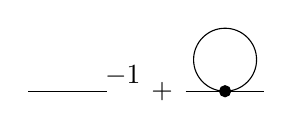
\begin{tikzpicture}[baseline=2ex]
           \draw (0,0.4) -- (1,0.4);
           \node at (1.2,0.6) {$-1$};
           \node at (1.7,0.4) {$+$};
           \draw (2,0.4) -- (3,0.4);
           \filldraw[black] (2.5,0.4) circle (2pt);
           \draw (2.5,0.8) circle (0.4);
       \end{tikzpicture}
\end{equation}
where
\begin{equation}
\Gamma_{0}^{\alpha \beta}(p)=-\left[G_{0}^{\alpha \beta}(p)\right]^{-1}=-\left(m_{0}^{2}+\hat{p}^{2}\right) \delta^{\alpha \beta}
\end{equation}
and
\begin{align}
\Gamma_{0}^{\alpha \beta \gamma{\delta}} & =-2 \lambda_{0} S_{\alpha \beta{\gamma} \delta}, \qquad S_{\alpha \beta \gamma  \delta}=\delta_{\alpha \beta} \delta_{\gamma \delta}+\delta_{\alpha \gamma} \delta_{\beta \delta}+\delta_{\alpha \delta} \delta_{\beta \gamma} 
\end{align}

\begin{align}
\Rightarrow \Gamma^{\alpha \beta}(p) & =-\left(m_{0}^{2}+\hat{p}^{2}\right)+\frac{1}{2}\left(-2 \lambda_{0} S_{\alpha \beta \gamma \delta}\right) \delta_{\gamma \delta} \int_{q} \frac{1}{m_{0}^{2}+\hat{q}^{2}} \\
& =-\delta_{\alpha \beta}\left[m_{0}^{2}+\hat{p}^{2}+\lambda_{0}(n+2) J_{1}\left(m_{0}\right)\right]
\end{align}
%
where $n$ arises from the contraction of $O(n)$ flavour indices and
%
\begin{equation}
J_{k}\left(m_{0}\right)=\int_{q} \frac{1}{\left(m_{0}^{2}+\hat{q}^{2}\right)^k}
\end{equation}
Similarly(see Fig.~\ref{fig:4pt1loop})
\begin{figure}
    \centering{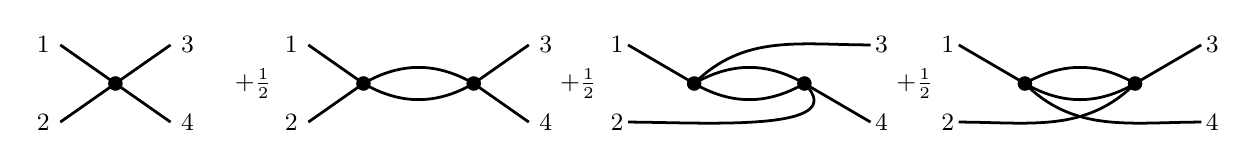
\begin{tikzpicture}[
    line width=1pt,
    every node/.style={font=\small,text=black},
    vertex/.style={draw, fill=black, circle, inner sep=1.5pt},
    extleg/.style={draw=black},
    intline/.style={draw=black},
    scale=0.7
  ]

  %--------------------------------------
  % 1) Tree‐level contact vertex at x=0
  %--------------------------------------
  \coordinate (V0) at (0,0);
  \node[vertex] at (V0) {};
  % External legs: 1 above, 2 below on left; 3 above, 4 below on right
  \draw[extleg] (V0) -- ++(-1.0,  0.7) node[left, text=black]  {1};
  \draw[extleg] (V0) -- ++(-1.0, -0.7) node[left, text=black]  {2};
  \draw[extleg] (V0) -- ++( 1.0,  0.7) node[right, text=black] {3};
  \draw[extleg] (V0) -- ++( 1.0, -0.7) node[right, text=black] {4};

  
  %--------------------------------------
  % 3) s‐channel one‐loop (at x≈4.5)
  %    • “1/2” multiplier
  %    • Two φ^4 vertices with 1,2 on left; 3,4 on right
  %--------------------------------------
  % 3a) the “1/2”
  \node at (2.5,  0) {$+ \frac{1}{2}$};

  % 3b) the s‐loop drawing
  \begin{scope}[shift={(4.5, 0)}]
    % Left φ^4 vertex
    \coordinate (Ls) at (0,0);
    \node[vertex] at (Ls) {};
    % Right φ^4 vertex
    \coordinate (Rs) at (2.0,0);
    \node[vertex] at (Rs) {};

    % External legs (no crossings in s‐channel)
    \draw[extleg] (Ls) -- ++(-1.0,  0.7) node[left, text=black]  {1};
    \draw[extleg] (Ls) -- ++(-1.0, -0.7) node[left, text=black]  {2};
    \draw[extleg] (Rs) -- ++( 1.0,  0.7) node[right, text=black] {3};
    \draw[extleg] (Rs) -- ++( 1.0, -0.7) node[right, text=black] {4};

    % Two internal propagators (forming the loop)
    \draw[intline] (Ls) to[out=30,  in=150] (Rs);
    \draw[intline] (Ls) to[out=-30, in=-150] (Rs);
  \end{scope}
  
  %--------------------------------------
  % 5) t‐channel one‐loop (at x≈9.5)
  %    • “+1/2” multiplier
  %    • External 1,2 on left; 3,4 on right but with crossings;
  %      labels moved further out
  %--------------------------------------
  % 5a) the “1/2”
  \node at (8.4, 0) {$+\frac{1}{2}$};

  % 5b) the t‐loop drawing
  \begin{scope}[shift={(10.5, 0)}]
    % Two φ^4 vertices at (0,0) and (2,0)
    \coordinate (Lt) at (0,0);
    \node[vertex] at (Lt) {};
    \coordinate (Rt) at (2,0);
    \node[vertex] at (Rt) {};

    % External node “gates” (moved farther from vertices):
    \coordinate (E1t) at (-1.2,  0.7); % 1 (left-top)
    \coordinate (E2t) at (-1.2, -0.7); % 2 (left-bottom)
    \coordinate (E3t) at (+3.2,  0.7); % 3 (right-top)
    \coordinate (E4t) at (+3.2, -0.7); % 4 (right-bottom)
    \coordinate (E1tx) at (-1.4,  0.7); % 1 (left-top)
    \coordinate (E2tx) at (-1.4, -0.7); % 2 (left-bottom)
    \coordinate (E3tx) at (+3.4,  0.7); % 3 (right-top)
    \coordinate (E4tx) at (+3.4, -0.7); % 4 (right-bottom)

    % Place labels
    \node at (E1tx) {1};
    \node at (E2tx) {2};
    \node at (E3tx) {3};
    \node at (E4tx) {4};


    % Connect 1 → Lt (straight)
    \draw[extleg] (E1t) -- (Lt);
    % Connect 3 → Lt (cross)
    \draw[extleg] (E3t) to[out=180, in=45] (Lt);
    % Connect 2 → Rt (cross under)
    \draw[extleg] (E2t) to[out=0, in=-45] (Rt);
    % Connect 4 → Rt (straight)
    \draw[extleg] (E4t) -- (Rt);

    % Two internal propagators forming the loop
    \draw[intline] (Lt) to[out=30,  in=150] (Rt);
    \draw[intline] (Lt) to[out=-30, in=-150] (Rt);
  \end{scope}

  
  %--------------------------------------
  % 7) u‐channel one‐loop (at x≈14.5)
  %    • “1/2” multiplier
  %    • External 1,2 on left; 3,4 on right with crossings;
  %      labels moved farther out
  %--------------------------------------
  % 7a) the “1/2”
  \node at (14.5, 0) {$+\frac{1}{2}$};

  % 7b) the u‐loop drawing
  \begin{scope}[shift={(16.5, 0)}]
    % Two φ^4 vertices at (0,0) and (2,0)
    \coordinate (Lu) at (0,0);
    \node[vertex] at (Lu) {};
    \coordinate (Ru) at (2,0);
    \node[vertex] at (Ru) {};

    % External node “gates”:
    \coordinate (E1u) at (-1.2,  0.7); % 1 (left-top)
    \coordinate (E2u) at (-1.2, -0.7); % 2 (left-bottom)
    \coordinate (E3u) at (+3.2,  0.7); % 3 (right-top)
    \coordinate (E4u) at (+3.2, -0.7); % 4 (right-bottom)
    \coordinate (E1ux) at (-1.4,  0.7); % 1 (left-top)
    \coordinate (E2ux) at (-1.4, -0.7); % 2 (left-bottom)
    \coordinate (E3ux) at (+3.4,  0.7); % 3 (right-top)
    \coordinate (E4ux) at (+3.4, -0.7); % 4 (right-bottom)

    % Place labels
    \node at (E1ux) {1};
    \node at (E2ux) {2};
    \node at (E3ux) {3};
    \node at (E4ux) {4};

    % Connect 1 → Lu (straight)
    \draw[extleg] (E1u) -- (Lu);
    % Connect 4 → Lu (cross back)
    \draw[extleg] (E4u) to[out=180, in=-45] (Lu);
    % Connect 2 → Ru (cross up)
    \draw[extleg] (E2u) to[out=0, in=-135] (Ru);
    % Connect 3 → Ru (straight)
    \draw[extleg] (E3u) -- (Ru);

    % Two internal propagators forming the loop
    \draw[intline] (Lu) to[out=30,  in=150] (Ru);
    \draw[intline] (Lu) to[out=-30, in=-150] (Ru);
  \end{scope}

\end{tikzpicture}
}
    \caption{The one-loop contributions to Eq.~\eqref{eq:1loop4pt}.
    \label{fig:4pt1loop}}
\end{figure}
\begin{equation}
\label{eq:1loop4pt}
\begin{aligned}
 \Gamma^{\alpha_{1} \ldots \alpha_{4}}\left(p_{1}, \ldots p_{4}\right)=&\Gamma_{0}^{\alpha_{1} \ldots \alpha_{4}}\left(p_{1} \ldots p_{4}\right) \\
& +\frac{1}{2} \int_{q} \Gamma_{0}^{\alpha_{1} \alpha_{2} \alpha_{5} \alpha_{6}}\left(p_{1}, p_{2}, q, p_{1}+p_{2}-q\right) G_{0}^{\alpha_{5} \alpha_{7}}(q) G_{0}^{\alpha_{6} \alpha_{8}}\left(p_{1}+p_{2}-q\right) \Gamma_{0}^{\alpha_{7} \alpha_{8} \alpha_{3} \alpha_{4}}\left(q, p_{3}+p_{4}-q, p_{3}, p_{4}\right) \\
& +2 \text { permutations }[(1,2,3,4) \rightarrow(1,3,2,4),(1,4,2,3)]\\
 =&-2 \lambda_{0} S_{\alpha_{1} \ldots \alpha_{4}}+\frac{1}{2}\left(-2 \lambda_{0}\right)^{2} S_{\alpha_{1} \alpha_{2} \alpha_{5} \alpha_{6}} S_{\alpha_{7} \alpha_{8} \alpha_{3} \alpha_{4}} \delta_{\alpha_{5} \alpha_{7}} \delta_{\alpha_{6} \alpha_{8}} \int_{q} \frac{1}{m_{0}^{2}+\hat{q}^{2}} \frac{1}{m_{0}^{2}+2 \sum_{\mu}\left(1-\cos \left(q+p_1+p_{2}\right)_{\mu}\right)} \\
& +2 \text { permutations }\\
=&-2 \lambda_{0} S_{\alpha_{1} \ldots \alpha_{4}}+2 \lambda_{0}^{2}\left\{t_{\alpha_{1} \alpha_{2} \alpha_{3} \alpha_{4}} I_{2}\left(m_{0}, p_{1}+p_{2}\right)+t_{\alpha_1 \alpha_{3} \alpha_{2} \alpha_{4}} I_{2}\left(m_{0}, p_{1}+p_{3}\right)+t_{\alpha_{1} \alpha_{4} \alpha_{2} \alpha_{3}} I_{2}\left(m_{0}, p_{1}+p_{4}\right)\right\}
\end{aligned}
\end{equation}
%
where \(t_{\alpha_{1} \ldots \alpha_{4}}=S_{\alpha_{1} \alpha_{2} \alpha_{5} \alpha_{6}} S_{\alpha_{5} \alpha_{6} \alpha_{3} \alpha_{4}}=\delta_{\alpha_{1} \alpha_{2}} \delta_{\alpha_{3} \alpha_{4}}(n+4)+2 \delta_{\alpha_{1} \alpha_{3}}\delta_{ \alpha_{2} \alpha_{4}}+2 \delta_{\alpha_{1} \alpha_{4}} \delta_{\alpha_{2} \alpha_{3}}\)\\
and
%
\begin{equation}
I_{2}\left(m_{0}, p\right)=\int_{q} \frac{1}{m_{0}^{2}+\hat{q}^{2}} \frac{1}{m_{0}^{2}+\widehat{p-q}^{2}}
\end{equation}

\begin{itemize}
  \item Lattice regulated integrals are quite ugly and need different techniques to dim. reg., e.g. in \(D=4\)
\end{itemize}
%
\begin{equation}
\begin{aligned}
& J_{1}\left(a m_{0}\right)=\int_{q} \frac{1}{\left(a m_{0}\right)^{2}+2 \sum_{\mu}\left(1-\cos q_{\mu}a\right)}
\end{aligned}
\end{equation}
%
which we can expand around \(a \rightarrow 0\), after using $1 - \cos x = 2 \sin^2 \frac{x}{2}$
%
\begin{equation}
\begin{aligned}
& J_{1}(m_0 a)=J_{1}(0)-a^{2} m_{0}^{2} \int_{q} \frac{1}{\left(4 \sum_{\mu} \sin ^{2}\left(\frac{q_\mu a}{2} \right)\right)} \frac{1}{\left(a^{2} m_{0}^{2}+4 \sum_{\nu} \sin ^{2}\left(\frac{q_\nu a}{2}\right)\right)}
\end{aligned}
\end{equation}

[use \(\frac{1}{m^{2}+x^{2}}=\frac{1}{x^{2}}-\frac{m^{2}}{x^{2}\left(m^{2}+x^{2}\right)}\) ]\\
where the \(J_{1}(0)\) integral is convergent - numerical evaluation gives

\begin{equation}
J_{1}(0)=r_{0}=0.15493338988 \ldots
\end{equation}

The second integral is IR divergent if $a m_0 \rightarrow 0$ so we need to account for that by looking at the continuum version ($x=q^2$)

\begin{equation}
    \int \frac{d^4q}{(2 \pi)^4}\frac{1}{q^2(m^2 + q^2)} = \int_0^\Lambda \frac{q^3 \text{d} q}{(2 \pi)^4} \int \text{d}\Omega \frac{1}{q^2(q^2+m^2)} = \int_0^{\Lambda^2} \frac{1}{16 \pi^2} \frac{x \text{d}x}{x(x+m^2)} = \frac{1}{16 \pi^2}\log \frac{\Lambda^2 + m^2}{m^2}
\end{equation}

So the following quantity is finite and numerically evaluatable

\begin{equation}
\begin{aligned}
& - {\left[\int_{q} \frac{1}{\hat{q}^{2}\left(\hat{q}^{2}+m^{2}\right)}+\frac{1}{16 \pi^{2}} \ln \left(m^{2}\right)\right]=r_{1}=-0.030345755 \ldots } \\
\Rightarrow & J_{1}\left(m_{0} a\right)=r_{0}+a^{2} m_{0}^{2}\left(\frac{1}{16 \pi^{2}} \ln \left(a^{2} m_{0}^{2}\right)+r_{1}\right)+{\cal O}\left(\left(a m_{0}\right)^{4}\right)
\end{aligned}
\end{equation}

Using similar techniques

\begin{equation}
I_{2}\left(a m_{0}, a p\right)=-r_{1}-\frac{1}{16\pi^{2}}\left(1+\int_{0}^{1} d x \ln \left\{a^{2}\left(m_0^{2}+x(1-x) p^{2}\right)\right\}\right)+{\cal O}\left(\left(a m_{0}\right)^{2}, a^{2} p^{2}\right)
\end{equation}

Thus
%
\begin{equation}
\begin{aligned}
&  \Gamma^{\alpha \beta}(p)=-\delta_{\alpha \beta}\left[m_{0}^{2}+\hat p^{2}+\lambda_{0}(n+2)\left\{\frac{r_{0}}{a^{2}}+r_{1} m_{0}^{2}+\frac{m_{0}^{2}}{16 \pi^{2}} \ln \left(a^{2} m_{0}^{2}\right)\right\}\right] \\
& \Gamma^{\alpha_{1} \ldots \alpha_{4}}\left(p_1, \ldots p_{4}\right)=-2 \lambda_{0} S_{\alpha_{1} \ldots \alpha_{4}}-2 \lambda_{0}^{2} t_{\alpha_{1} \ldots \alpha_{4}}\left\{r_{1}+\frac{1}{16 \pi^{2}}\left(1+\int_{0}^{1} d x \ln \left[a^{2}\left(m_{0}^{2}+x(1-x)\left(p_{1}+p_{2}\right)^{2}\right)\right]\right)\right\}\\
& \qquad \qquad \qquad \qquad \qquad+ \text{two permutations}
\end{aligned}
\end{equation}

\begin{itemize}
  \item Renormalisation: renormalised quantities should be regulator independent
  \begin{itemize}
      \item In this theory, there are two couplings and a field renormalization
      \item The two-point vertex function fixes $Z$ and $m_R$ (recall that $\Gamma^R_{(n)} = Z^{n/2}\Gamma_{(n)}$)
  \end{itemize}

\begin{equation}
    \Gamma^{\alpha \beta}(p) = - Z^{-1}(p^2 + m^2_R + O(p^4))\delta_{\alpha \beta}  
\end{equation}

    \begin{itemize}
        \item Since the one-loop diagram contributing to the two-point function is momentum independent, 
        \begin{equation}
            Z = 1 + O(\lambda_0^2),
        \end{equation}
        with the latter contributions starting at two loops, and
    \end{itemize}

\begin{align}
    m_R^2 &= m_0^2 + \lambda_0(n+2) \left\{\frac{r_0}{a^2} + r_1 m_0^2 + \frac{m_0^2}{16 \pi^2}\log(a^2 m_0^2) \right\} + O(\lambda_0^2)
\end{align}
and thus 
    \begin{align}
    m_0^2&= m_R^2 - \lambda_R(n+2) \left\{\frac{r_0}{a^2} - r_1 m_R^2 + \frac{m_R^2}{16 \pi^2}\log(a^2 m_0^2) \right\} + O(\lambda_R^2)
    \label{eq:m0vsmR}
\end{align}

\begin{itemize}
 \item To fix \(\lambda_{R}\), demand
\end{itemize}

\begin{align}
    Z^2 &\Gamma_{\alpha_1 \ldots \alpha_4}(0,0,0,0) =  \Gamma_{\alpha_1 \ldots \alpha_4}^R(0,0,0,0) = -2 \lambda_R S_{\alpha_1 \ldots \alpha_4}\\
    &= (1 + {\cal O}(\lambda_0)^2)^2\left[-2 \lambda_0 S_{\alpha_1 \ldots \alpha_4} - 2 \lambda_0^2\left(t_{\alpha_1 \alpha_2 \alpha_3 \alpha_4} + t_{\alpha_1 \alpha_3 \alpha_2 \alpha_4} + t_{\alpha_1 \alpha_4 \alpha_2 \alpha_3}\right)\left(r_1 + \frac{1}{16 \pi^2}\left(1 + \log(a^2 m_0^2)\right)\right)\right]\\
    &\Rightarrow \lambda_R = \lambda_0 + \lambda_0^2 \frac{(n+8)}{16 \pi^2}(\log(a^2 m_0^2) + 16 \pi^2 r_1 + 1) + O(\lambda_0^3)\\
    &\Rightarrow \lambda_0 = \lambda_R - \lambda_R^2 \frac{n+8}{16 \pi^2}(\log(a^2 m_R^2) + 16 \pi^2 r_1 + 1)+ O(\lambda_R^3)
\end{align}
using $\left(t_{\alpha_1 \alpha_2 \alpha_3 \alpha_4} + t_{\alpha_1 \alpha_3 \alpha_2 \alpha_4} + t_{\alpha_1 \alpha_4 \alpha_2 \alpha_3}\right)=(n+8) S_{\alpha_1\alpha_2\alpha_3\alpha_4}$.
\item Gives renormalized vertex functions
\begin{equation}
    \Gamma^R_{\alpha \beta} = -\delta_{\alpha \beta}(\hat p^2 + m^2_R) + O(\lambda_R^2)
\end{equation}
\begin{align}
    \Gamma^R_{\alpha_1 \ldots \alpha_4}(p_1, \ldots, p_4) =& -2 \lambda_R S_{\alpha_1 \ldots \alpha_4} + 2 \lambda_R^2 S_{\alpha_1 \ldots \alpha_4}\frac{n+8}{16 \pi^2}(\log a^2 m_R^2 + 16 \pi^2 r_1 + 1)\\
    &-2 \lambda_R^2 t_{\alpha_1 \ldots \alpha_4}\left\{ r_1 + \frac{1}{16 \pi^2}\left(1 + \int_0^1 \text{d}x \log\left[a^2(m_R^2 + x(1-x)(p_1 + p_2)^2)\right]\right)\right\} + \text{2 perms} \\
    =& - 2 \lambda_R S_{\alpha_1 \ldots \alpha_4} - \frac{2 \lambda_R^2}{16 \pi^2}t_{\alpha_1 \ldots \alpha_4} \int_0^1 \text{d}x \log \left[ \frac{m_R^2 + x(1-x)(p_1 + p_2)^2}{m_R^2}\right] + \text{2 perms} + O(\lambda_R^3)
\end{align}
which are independent of $a$ and of $r_0, r_1$ (which are regulator artifacts)
\item Weak coupling expansion describes the theory for small $\lambda_0, \lambda_R$ and we can already make statements about the field theory in the continuum limit for this region, for example computing the $\beta$-function, but let's learn more first
\end{itemize}

\section{Hopping expansion (aka: high temperature expansion)} 
\begin{itemize}
 \item As discussed above, can rewrite action as

\begin{align}
S&=\sum_{n}\left\{-2 \kappa \sum_{\mu} \phi_{n}^{a} \phi_{n+\hat{\mu}}^{a}+\phi_{n}^{a 2}+\lambda\left(\phi_{n}^{a 2}-1\right)^{2}-\lambda\right\}\\
&= \sum_n s(\phi_n) - 2 \kappa \sum_{\langle n, m\rangle}\phi_n \phi_m
\end{align}
where
\begin{equation}
    s(\phi_n)=\phi_n^{a 2}+\lambda(\phi_n^{a2}-1)^2 -\lambda
\end{equation}
with \(a \varphi_{n}^{a}=\sqrt{2 \kappa} \phi_{n}^{a}, a^{2} m_{0}^{2}=\frac{1-2 \lambda}{\kappa}-2(d+1), \lambda_{0}=\frac{\lambda}{\kappa^{2}}\) and the sum runs over all neighbors

\item Correlation functions can therefore be evaluated as

\begin{equation}
\begin{aligned}
\left\langle\phi_{n_{1}}\ldots \phi_{n_k}\right\rangle & =\frac{1}{Z} \int \mathcal{D} \phi e^{-S} \phi_{n_{1}}\ldots \phi_{n_k} \\
& =\frac{1}{Z} \int \mathcal{D} \phi\left[\prod_{n} e^{-s\left(\phi_{n}\right)}\right] \exp\left[2 \kappa \sum_{\langle n, m\rangle} \phi_{n} \phi_{m}\right] \phi_{n_1} \ldots \phi_{n_k} \\
& =\frac{1}{Z} \sum_{j}\frac{(2 \kappa)^{j}}{j!} \int \mathcal{D} \phi \prod_{n} e^{-s\left(\phi_{n}\right)}\left(\sum_{\langle n, m\rangle} \phi_{n} \phi_{m}\right)^{j} \phi_{n_1}\ldots \phi_{n_k}
\end{aligned}
\end{equation}

which can be shown to have a non-zero radius of convergence in $\kappa$ for any fixed coupling $\lambda$.
See Fig.~\ref{fig:kappa_exp}.
\begin{figure}
    \centering
    
\includegraphics[width=0.5\linewidth]{fig-notes-094.pdf}
    \caption{Phae diagram region studied in hopping explansion. 
    \label{fig:kappa_exp}}
\end{figure}

\item E.g. $Z = Z_0 + Z_1 + Z_2 + \ldots$ where $Z_i\sim \kappa^i$


\begin{equation}
\begin{aligned}
Z_{0} & =\int \mathcal{D} \phi\left[\prod_{n} e^{-s\left(\phi_{n}\right)} \right]=\prod_{n} \int d \phi_{n} e^{-s\left(\phi_{n}\right)} \\
& =\left(\int d \phi e^{-s(\phi)}\right)^{\Omega}=z_{0}^{\Omega} 
\end{aligned}
\end{equation}
where $z_0$ is the single site partition function and $\Omega$ is the total number of sites.

\begin{equation}
\begin{aligned}
& Z_{1}=2 \kappa \prod_{n} \int d \phi_{n} e^{-s\left(\phi_{n}\right)} \sum_{\langle l, m\rangle} \phi_{l} \phi_{m} \\
& =2 \kappa z_{0}^{\Omega - 2} \sum_{\langle l, m\rangle}\underbrace{\int d \phi_{l} e^{-s\left(\phi_{l}\right)} \phi_{l}}_{=0}\ \underbrace{\int d \phi_{m} e^{-s\left(\phi_{m}\right)} \phi_{m}}_{=0}, \qquad m \neq l \\
& =0
\end{aligned}
\end{equation}

\begin{equation}
\begin{aligned}
& Z_{2}=\frac{(2 \kappa)^{2}}{2} \prod_{n} \int d \phi_{n} e^{-s\left(\phi_{n}\right)}\left[\sum_{\langle l, m\rangle} \phi_{l} \phi_{m}\right]\left[\sum_{\langle p,q \rangle} \phi_{p} \phi_{q}\right] \\
&\quad \; \,= \frac{(2\kappa)^2}{2}z_0^\Omega \{ A \underbrace{\gamma_1^4}_{p \neq q \neq l \neq m} + B \underbrace{\gamma_1^2 \gamma_2}_{p = l \neq q \neq m} + C \underbrace{\gamma_2^2}_{p=l, q = m} \}
\end{aligned}
\end{equation}

\begin{itemize}
    \item where 
    \begin{equation}
        \gamma_n = \gamma_n(\lambda) = \frac{1}{z_0} \int \text{d}\phi e^{-s(\phi)}\phi^n
    \end{equation}
    \item which are generated by 
    \begin{equation}
        z(j) = z_0^{-1}\int \text{d}\phi e^{-s(\phi) + j \phi} = \sum_{k=0}^\infty \frac{1}{k!} j^k \gamma_k
    \end{equation}
    \item Note that $\gamma_n$ depends on $\lambda$ and can be evaluated numerically and vanishes for odd $n$, and that $A, B, C$ can be found by considering Fig.~\ref{fig:hopping_Z2} (in $D=4$)
\end{itemize}

\begin{figure}
    \centering
    \redrawcompare{fig-notes-006.jpg}{fig-redraw-006.pdf}
    \caption{Potential contributions to $Z_2$ (A, B, C from left to right).
    \label{fig:hopping_Z2}}
\end{figure}

\begin{equation}
\begin{aligned}
A & =4 \Omega \times\left\{\begin{array}{l}
4(\Omega-5) \\
+3\\
+2.3 .3
\end{array}, 
\quad B=\Omega \times \frac{4 \times 3}{2},
\quad C=4 \Omega=\#\right. \text { links }
\end{aligned}
\end{equation}
Thus
\begin{equation}
 Z_{2}  =\frac{(2 \kappa)^{2}}{2} z_{0}^{\Omega} 4 \Omega \gamma_{2}^{2}.
\end{equation}

\begin{itemize}
  \item Clearly \(\mathrm{Z}_{3}=0\) as must involve the terms in Fig.~\ref{fig:hopping_Z3} each of which is zero because it involves $\gamma_j$ for odd $j$.
\end{itemize}

\begin{figure}
    \centering
    \redrawcompare{fig-notes-054.png}{fig-redraw-054.pdf}
    \caption{Potential contributions to $Z_3$ (all vanish).
    \label{fig:hopping_Z3}}
\end{figure}



\begin{itemize}
  \item For \(\mathrm{Z}_{4}\), non-vanishing contributions are shown in Fig.~\ref{fig:hopping_Z4}
\end{itemize}
\begin{figure}
    \centering
    \redrawcompare{fig-notes-055.png}{fig-redraw-055.pdf}
    \caption{Potential contributions to $Z_4$.
    \label{fig:hopping_Z4}}
\end{figure}

\begin{equation}
    \Rightarrow Z_4 = (2 \kappa)^4 z_0^\Omega \{ \gamma_4^2 \frac{\Omega}{6} + \gamma_2^2 \gamma_4 7 \Omega + \gamma_2^4 \Omega\left(6 + \frac{4 \Omega - 15}{2}\right)\}
\end{equation}
\\

\begin{itemize}
  \item To learn about renormalisation, need to compute the following (ie propagator and 4-point vertex)

\begin{equation}
\begin{aligned}
& \chi_{2}(\lambda,\kappa)=\left\langle\sum_{m} \phi_{m} \phi_{0}\right\rangle_{\text{conn}} \\
& =Z^{-1}\left[\prod_{n} \int d \phi_{n} e^{-s\left(\phi_{n}\right)}\right] e^{2 \kappa \sum_{\langle p,q\rangle} \phi_{p} \phi_{q}} \sum_{m} \phi_{m} \phi_{0}=
 \gamma_{2}+(2 \kappa) 8 \gamma_{2}^{2} 
 +(2 \kappa)^{2}\left(56 \gamma_{2}^{3}+4 \gamma_{2}\left(\gamma_{4}-\gamma_{2}^{2}\right)\right) 
 +O\left(\kappa^{3}\right)
\end{aligned}
\end{equation}

\item as well as
\end{itemize}

\begin{equation}
\mu_{2}(\lambda,\kappa)=\left\langle\sum_{m} m^{2} \phi_{m} \phi_{0}\right\rangle_{\text {conn }}=2 \kappa 8 \gamma_{2}^{2}+(2 \kappa)^{2} 128 \gamma_{2}^{3}+O\left(\kappa^{3}\right)
\end{equation}

and

\begin{equation}
\chi_{4}(\lambda,\kappa)=\left\langle\sum_{l, m, n} \phi_{l} \phi_{m} \phi_{n} \phi_{0}\right\rangle_{\text{conn}}=\left(\gamma_{4}-3 \gamma_{2}^{2}\right)+2 \kappa 32 \gamma_{2}\left(\gamma_{4}-3 \gamma_{2}^{2}\right)+O\left(\kappa^{2}\right)
\end{equation}
\begin{itemize}
\item These can easily be related to \(m_{R}, Z_{R}, \lambda_{R}\)
\end{itemize}

\begin{equation}
m_{R}^{2}(\lambda,\kappa)=2D \frac{\chi_{2}}{\mu_{2}}, \qquad Z_{R}(\lambda,\kappa)=2 D \frac{\chi_{2}^{2}}{\mu_{2}}, \qquad \lambda_{R}(\lambda,\kappa)=-(2 D)^{2} \frac{\chi_{4}}{\mu_{2}^{2}}
\end{equation}

\begin{itemize}
  \item In a powerful set of papers, L\"uscher and  Weisz (1987-9) calculated there quantities to \(O\left(\kappa^{14}\right)\), thereby controlling \(\beta\)-func for all \(\kappa<0.95 \kappa_{c}\) to \(O(1\%)\) uncertainty [This required a lot of graph theoretic reasoning and automation]\\
Thus we know renormalized quantities in the region shown in Fig.~\ref{fig:hoppdiag2}
\begin{figure}
    \centering
    \redrawcompare{fig-notes-007.jpg}{fig-redraw-007.pdf}
    \caption{Region of $O(n)$ phase diagram controlled by the hopping expansion.
    \label{fig:hoppdiag2}}
\end{figure}
and at \(\kappa / \kappa_{c}=0.95, m_{R}\) and \(g_{R}\) are monotonic with
\end{itemize}

\begin{center}
\begin{tabular}{c|cc}
\(\lambda_0\) & 0 & \(\infty\) \\
\hline
\(m_{R}\) & 0.65 & 0.49 \\
\(\lambda_{R}\) & 0 & 41 \\
\end{tabular}
\end{center}

\begin{itemize}
  \item Since \(m_{R}=\overline{m_{R}} a<1\), cutoff effects are mild (and get smaller as $\kappa\to\kappa_c$) so at \(\kappa / \kappa_{c}=0.95\) are in scaling region
\item Since $\lambda_R/(16\pi^2)\lesssim 1/3$, renormalised perturbation theory works in this regime (even though $\lambda_0\to\infty$!)
\item L\&W showed that with 3 loop calculations, errors are $<1$\%.
\end{itemize}
\end{itemize}




\section{Renormalisation group equations and the continuum limit}

Recall the relation between bare and renormalised quantities

\begin{equation}
\sqrt{Z} \phi_{R}=\phi_{0}, \quad \Gamma_{R}^{(n)}=Z^{n / 2} \Gamma_{0}^{(n)}
\end{equation}

with \(Z, m_{R}\) and \(\lambda_{R}\) defined by

\begin{equation}
\left.\frac{\partial^{2}}{\partial p^{2}} \Gamma_{R}^{(2)}(p)\right|_{p=0}=-Z, \quad \Gamma_{R}^{(2)}(0)=-m_{R}^{2}, \quad \Gamma_{R}^{(4)}(0,0,0,0)=-2 \lambda_{R}=-g_{R}
\end{equation}
(we will use $g_R$ to be generic here)
\begin{itemize}
  \item ``Wilson (-Kadanoff)''-like RGE

Wilsonian approach to RG is how does action change (infinite \# couplings) as modes are integrated out to leave low energy physics unchanged.

Consider the set of bare theories with the same renormalized $g_R$ - these define a one parameter subspace in the $m_0 a$, $\lambda_0 \sim g_0$ plane and every point on it has a different $m_R a = \frac{1}{\Lambda}$, where $\Lambda$ is the cutoff. $m_R a$ is then a dimensionless quantity characterizing the cutoff.

Renormalized vertex functions differ from the continuum limit by scaling violations
\begin{equation}
    \Gamma_R^{(n)} (\ldots, m_R a) = \Gamma_R^{(n)}(\ldots, 0) + \mathcal{O}(a^2 (\log a)^k),
\end{equation}
if working to $k$ loops, so 
\begin{equation}
    m_R a \frac{\text{d}}{\text{d} m_R a} \Gamma_R = a \frac{\text{d}}{\text{d}a} \Gamma_R^{(n)}(p_i, g_R, m_R, m_Ra) = 0 + \mathcal{O}(a^2 (\log a)^k).
\end{equation}
where the $m_Ra$-dependence is really showing dependence on the cutoff in dimensionless way.
Neglecting scaling violations and writing
\begin{align}
    &\Gamma^{(n)} = Z^{n/2}(g_0, m_Ra)\Gamma_0^{(n)}(g_0, m_R, m_R a) \nonumber \\
    \Rightarrow &\left\{a \frac{\partial}{\partial a} + \beta_{WK} \frac{\partial}{\partial g_0} + n \gamma_{WK} \right\} \Gamma_0^{(n)}(g_0, m_R, m_R a) = 0.
\end{align}

where

\begin{align}
    \beta_{WK}(g_0, m_R a) &= - a \frac{\partial g_0}{\partial a}\bigg|_{g_R \, \text{fixed}}\\
    &= -m_R a \left.\frac{\partial g_0}{\partial m_Ra}\right|_{g_R\text{ fixed}}
    =-\left.\frac{\partial g_0}{\partial \ln(m_Ra)}\right|_{g_R\text{ fixed}}
    \\
    \gamma_{WK}(g_0, m_R a) &= \frac{1}{2} a \frac{\partial \log Z}{\partial a}\bigg|_{g_R \, \text{fixed}}
\end{align}

The dependence on \(m_{R} a\) comes only from scaling violations. \(\beta_{WK}(g_0)\) controls how $g_0$ changes with the cutoff.


  \item Callan-Symanzik RGE


How does renorm coupling change as cutoff changes for fixed bare coupling?

\begin{align}
    m_R \frac{\text{d}}{\text{d} m_R}\Gamma^{(n)}_R(p_i, g_R, m_R, m_R a) =  m_R \frac{\partial}{\partial m_R}\Gamma^{(n)}_R + m_R \frac{\partial g_R}{\partial m_R} \frac{\partial}{\partial g_R}\Gamma^{(n)}_R \\
    = m_R \frac{\text{d}}{\text{d} m_R} (Z^{n/2}\Gamma^{(n)}) = \frac{n}{2}m_R \frac{\partial}{\partial m_R}(\log Z)\Gamma^{(n)}_R + Z^{n/2}m_R \frac{\partial}{\partial m_R}\Gamma^{(n)},
\end{align}
all evaluated at fixed bare coupling $g_0$. This implies
\begin{equation}
\label{eq:CS_rge}
    \left\{ m_R \frac{\partial}{\partial m_R} + \beta_{CS}\frac{\partial}{\partial g_R} - n \gamma_{CS}\right\} \Gamma_R^{(n)} = \frac{Z^{n/2}}{2}\frac{\partial}{\partial m_R^2}\Gamma^{(n)}
\end{equation}

where
\begin{align}
    \beta_{CS}(g_R, m_R a) &= m_R \frac{\partial g_R}{\partial m_R}\bigg|_{g_0\text{ fixed}} \\
    \gamma_{CS}(g_R, m_R a) &= \frac{1}{2}m_R \frac{\partial \log Z}{\partial m_R}\bigg|_{g_0\text{ fixed}}.
\end{align}
Furthermore, we can express $\beta_{CS}$ as
\begin{equation}
    \beta_{CS} = b \frac{\partial g}{\partial b} = a \frac{\partial g}{\partial a},
\end{equation}
where $b \equiv m_R a$, as can be checked through judicious application of the chain rule.
%
The RHS of Eq.~\eqref{eq:CS_rge} is actually the renormalized vertex function with one additional insertion of $m_R^2 \phi_R^2$, as you can see diagrammatically; this implies that the RHS is finite as $a \rightarrow 0$.
%
Since the LHS involves derivatives of renormalized vertex functions, which are also finite in this limit, $\beta_{CS}$ and $\gamma_{CS}$ must have continuum limits, and since they are dimensionless they are independent of $m_R a$ up to scaling violations.
%

    \item The two types of beta functions are related
\end{itemize}
\begin{align}
    0 = a \frac{\text{d}}{\text{d}a} g_R(g_0, m_R a) &= \left \{ a \frac{\partial}{\partial a} + a \frac{\partial g_0}{\partial a} \frac{\partial}{\partial g_0}\right \} g_R \nonumber \\
    &= m_R \frac{\partial}{\partial m_R}g_R + a \frac{\partial g_0}{\partial a} \frac{\partial g_R}{\partial g_0} \nonumber \\
    &= \beta_{CS}(g_R) - \beta_{WK}(g_0) \frac{\partial g_R}{\partial g_0} \nonumber \\
    \Rightarrow \beta_{WK}\frac{\partial g_R}{\partial g_0} &= \beta_{CS}.
\end{align}
\begin{itemize}
    \item The $\beta$ functions tell us how the bare (WK) and renormalised (CS) couplings behave as the continuum limit is taken
\begin{equation}
    \beta_{CS}(g_R) = m_R a \frac{\partial g_R}{\partial m_R a}\bigg|_{g_0} = \frac{\partial g_R}{\partial \log(m_R a)}\bigg|_{g_0}, \quad \beta_{WK}(g_0) = -\frac{\partial g_0}{\partial \log (m_R a)}\bigg|_{g_R}
\end{equation}

\item Potential behaviour that would allow a continuum theory is shown in Fig.~\ref{fig:potential_flow}.
\end{itemize}
\begin{figure}
    \centering
    
\includegraphics[width=0.45\linewidth]{fig-notes-091.pdf}\qquad
    
\includegraphics[width=0.45\linewidth]{fig-notes-092.pdf}
    \caption{Left: Potential $\beta_{CS}(g_R)$, with two IR fixed points where theory converges as cutoff $\to\infty$ and one UV fixed point which repels as cutoff is taken away.
    Right: The flow is opposite for $\beta_{WK}$. Given the same fixed point structure, the flow in terms of the bare parameters is shown. For $g_1\leq g_R \leq g_3$, the curves reach $m_R a=0$ so have a continuum limit.
    \label{fig:potential_flow}}
\end{figure}
\begin{itemize}
  \item In the regime of $g_R \rightarrow 0$, $\beta_{CS}$ and $\gamma_{CS}$ can be computed in renormalized perturbation theory. Close to $a \rightarrow 0$ this can be done in the continuum theory
\end{itemize}

\begin{equation}
\label{eq:continuum_limit_beta_cs}
    \beta_{CS}(g_R) = \beta_1 g_R^2 + \beta_2 g_R^3 + \ldots,
\end{equation}
and similarly for $\gamma$. For $O(1)$ in $4$D
\begin{equation}
    \beta_1 = \frac{3}{16 \pi^2} \quad \beta_2 = - \frac{17}{768 \pi^4}
\end{equation}
Since $g_R = g_0 + \mathcal{O}(g_0^2)$, $\beta_{WK}(g_0) = \hat{\beta}_1 g_0^2 + \hat{\beta}_2 g_0^3 + \ldots$, with $\hat{\beta}_1 = \beta_1$ and $\hat{\beta}_2 = \beta_2$ but $\hat{\beta}_3 \neq \beta_3$ (i.e. only the first two coefficients are universal).

\begin{itemize}
    \item The signs on $\beta_1$ show that $g_R = g_0 = 0$ is an IR fixed point, and solving the CS equation:
\end{itemize}
\begin{align}
\label{eq:one-loop-RGE}
    &\frac{\partial \log m_R a}{\partial g_R} = \frac{1}{\beta_{CS}(g_R)} \Rightarrow \log(m_R a) = \int_{\hat{g}}^{g_R}\text{d} g^\prime \frac{1}{\beta_{CS}(g^\prime)}\nonumber \\
    &\Rightarrow m_R a = C e^{- \frac{1}{\beta_1 g_R}}(\beta_1 g_R)^{-\beta_2 / \beta_1^2} (1 + \mathcal{O}(g_R)) \Rightarrow g_R = \frac{1}{\beta_1 \log(C/m_R a)} \Rightarrow g_R \rightarrow 0 \, \text{as} \, a \rightarrow 0.
\end{align}

\begin{itemize}
  \item But Eq.~\eqref{eq:one-loop-RGE} only makes sense for $g_R \rightarrow 0$, what about larger values?
\end{itemize}
\(\Rightarrow\) Back to Lüscher-Weisz (LW) results\\
\begin{figure}
    \centering
    \redrawcompare{fig-notes-056.png}{fig-redraw-056.pdf}
    \caption{A schematic showing the range of applicability of the $\kappa$ expansion and how the RGE helps us to understand the continuum limit. Note that in the  variation of $\lambda_0$ from 0 to $\infty$ (horizontal axis), $\bar\lambda$ varies from 0 to 1.}
    \label{fig:enter-label}
\end{figure}

\begin{itemize}
    \item LW integrated RGE up to critical line for the region where the hopping parameter expansion is controlled, finding no other fixed points!!
    \item LW also showed through other techniques that we won't go into that the phase diagram is also controlled for $\kappa > \kappa_C$ in the scaling regime (and numerical calculations can be performed)
    \item Finally, curves of constant $\lambda_R$ take the form depicted in Fig.~\ref{fig:lam0_curves}. 
\end{itemize}
\begin{figure}
    \centering
    \redrawcompare{fig-notes-008.jpg}{fig-redraw-008.pdf}
    \caption{A schematic representation of the curves of constant $\lambda_R$. Only the $\lambda_R = 0$ curve admits a continuum limit.}
    \label{fig:lam0_curves}
\end{figure}

Note that LW use $\bar{\lambda} = - \frac{1}{2} \left(\frac{\gamma_4 - 3 \gamma_2^2}{\gamma_2^2}\right)$, which depends on $\lambda_0$ such that $\bar{\lambda} \sim 3 \lambda_0$ for $\lambda_0 \ll 1$ and $\bar{\lambda} \rightarrow 1$ as $\lambda_0 \rightarrow \infty$ monotonically. At $\bar{\lambda} = 1$, they find (Nucl Phys B295(1988) 65)

\begin{table}[h]
\centering
\begin{tabular}{c|c}
    $g_R$ & $m_R$ \\
    \hline
    $10$ & $0.01$ \\
    $15$ & $0.07$ \\
    $27$ & $0.4$ \\
    $31$ & $0.5$
\end{tabular}
\end{table}
In all cases except $\lambda_R = 0$, the bare coupling $\rightarrow \infty$ before the continuum limit is reached (i.e. reaches $\bar{\lambda} = 1$ for $\kappa < \kappa_C$, see Fig.~\ref{fig:On_beta_func_final}. This means that for any non-zero renormalized coupling, there is no continuum limit!!
\begin{figure}
    \centering
    \redrawcompare{fig-notes-057.png}{fig-redraw-057.pdf}
    \caption{Final $\beta$ function in $O(n)$ model.
    \label{fig:On_beta_func_final}}
\end{figure}
